\documentclass{standalone}
\usepackage{tikz}
\usetikzlibrary{patterns, positioning}


\begin{document}
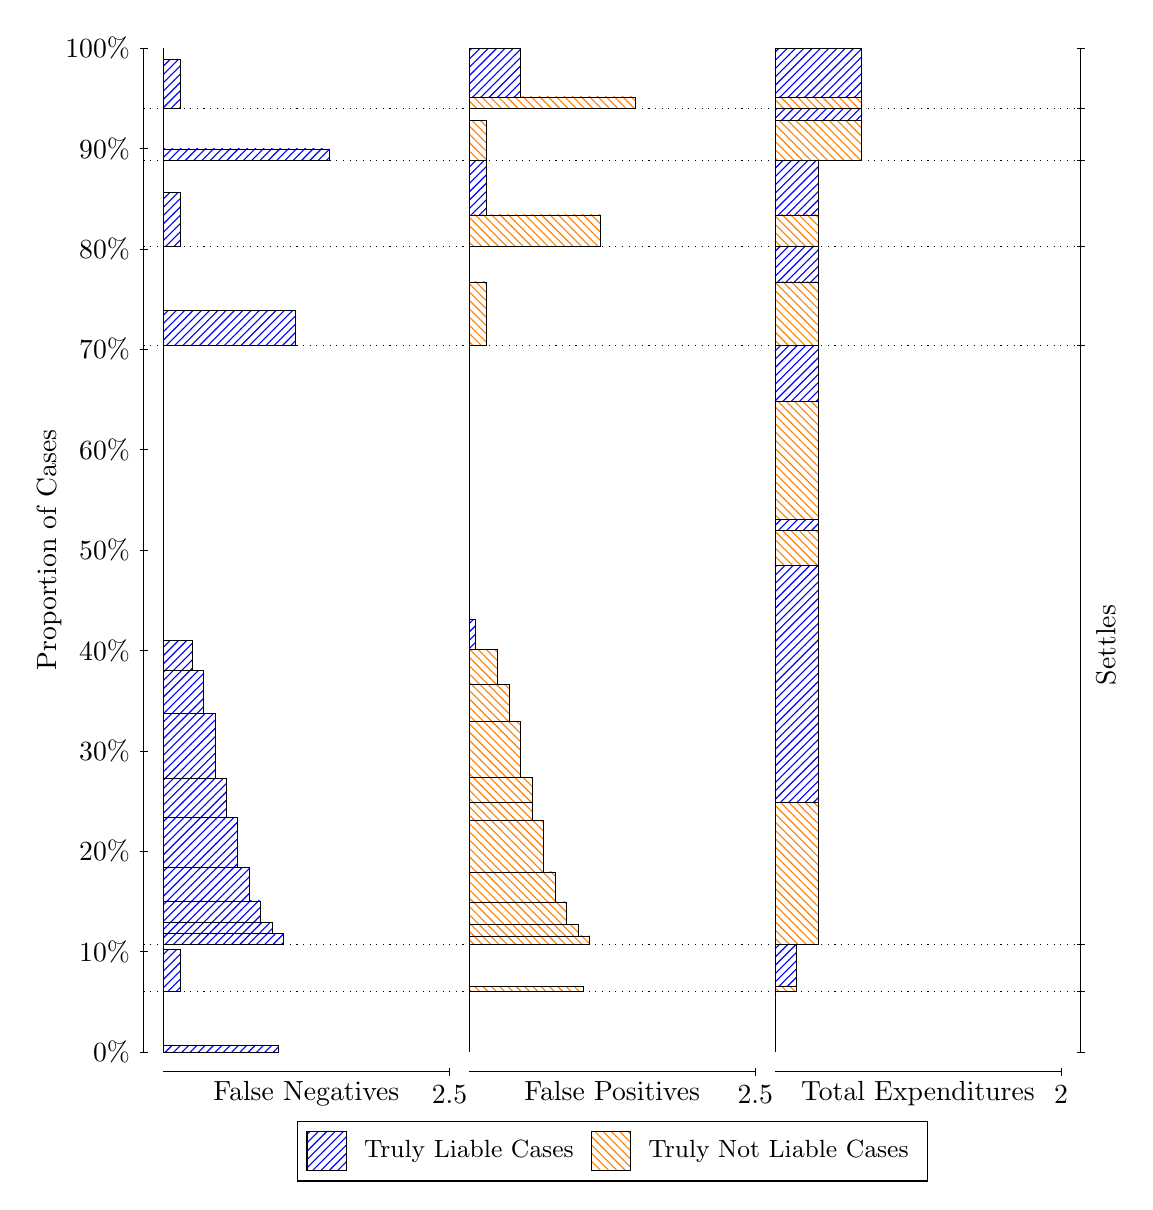
\begin{tikzpicture}
\draw[black, very thin] (1.5,1.75) -- (1.5,14.5);
\node[rotate=90, text=black, anchor=center] at (0.3, 8.125) {Proportion of Cases};
\draw[black, very thin] (1.45,1.75) -- (1.55,1.75);
\node[text=black, anchor=east] at (1.45, 1.75) {0\%};
\draw[black, very thin] (1.45,3.025) -- (1.55,3.025);
\node[text=black, anchor=east] at (1.45, 3.025) {10\%};
\draw[black, very thin] (1.45,4.3) -- (1.55,4.3);
\node[text=black, anchor=east] at (1.45, 4.3) {20\%};
\draw[black, very thin] (1.45,5.575) -- (1.55,5.575);
\node[text=black, anchor=east] at (1.45, 5.575) {30\%};
\draw[black, very thin] (1.45,6.85) -- (1.55,6.85);
\node[text=black, anchor=east] at (1.45, 6.85) {40\%};
\draw[black, very thin] (1.45,8.125) -- (1.55,8.125);
\node[text=black, anchor=east] at (1.45, 8.125) {50\%};
\draw[black, very thin] (1.45,9.4) -- (1.55,9.4);
\node[text=black, anchor=east] at (1.45, 9.4) {60\%};
\draw[black, very thin] (1.45,10.675) -- (1.55,10.675);
\node[text=black, anchor=east] at (1.45, 10.675) {70\%};
\draw[black, very thin] (1.45,11.95) -- (1.55,11.95);
\node[text=black, anchor=east] at (1.45, 11.95) {80\%};
\draw[black, very thin] (1.45,13.225) -- (1.55,13.225);
\node[text=black, anchor=east] at (1.45, 13.225) {90\%};
\draw[black, very thin] (1.45,14.5) -- (1.55,14.5);
\node[text=black, anchor=east] at (1.45, 14.5) {100\%};

\draw[black, very thin] (13.4,1.75) -- (13.4,14.5);
\draw[black, very thin] (13.35,1.75) -- (13.45,1.75);
\node[anchor=west] at (13.35, 1.75) {};
\draw[black, very thin] (13.35,2.5234) -- (13.45,2.5234);
\node[anchor=west] at (13.35, 2.5234) {};
\draw[black, very thin] (13.35,3.1128) -- (13.45,3.1128);
\node[anchor=west] at (13.35, 3.1128) {};
\draw[black, very thin] (13.35,10.721) -- (13.45,10.721);
\node[anchor=west] at (13.35, 10.721) {};
\draw[black, very thin] (13.35,11.977) -- (13.45,11.977);
\node[anchor=west] at (13.35, 11.977) {};
\draw[black, very thin] (13.35,13.07) -- (13.45,13.07);
\node[anchor=west] at (13.35, 13.07) {};
\draw[black, very thin] (13.35,13.73) -- (13.45,13.73);
\node[anchor=west] at (13.35, 13.73) {};
\draw[black, very thin] (13.35,14.5) -- (13.45,14.5);
\node[anchor=west] at (13.35, 14.5) {};

\draw[black, very thin, pattern color=blue, pattern=north east lines] (1.75,1.75) rectangle (3.2033,1.8314);
\draw[black, very thin, pattern color=orange, pattern=north west lines] (1.75,1.8314) rectangle (1.75,2.5234);
\draw[black, very thin, pattern color=blue, pattern=north east lines] (1.75,2.5234) rectangle (1.968,3.0513);
\draw[black, very thin, pattern color=orange, pattern=north west lines] (1.75,3.0513) rectangle (1.75,3.1128);
\draw[black, very thin, pattern color=blue, pattern=north east lines] (1.75,3.1128) rectangle (3.276,3.2526);
\draw[black, very thin, pattern color=blue, pattern=north east lines] (1.75,3.2526) rectangle (3.1307,3.3963);
\draw[black, very thin, pattern color=blue, pattern=north east lines] (1.75,3.3963) rectangle (2.9853,3.6679);
\draw[black, very thin, pattern color=blue, pattern=north east lines] (1.75,3.6679) rectangle (2.84,4.0896);
\draw[black, very thin, pattern color=blue, pattern=north east lines] (1.75,4.0896) rectangle (2.6947,4.7314);
\draw[black, very thin, pattern color=blue, pattern=north east lines] (1.75,4.7314) rectangle (2.5493,5.2244);
\draw[black, very thin, pattern color=blue, pattern=north east lines] (1.75,5.2244) rectangle (2.404,6.0529);
\draw[black, very thin, pattern color=blue, pattern=north east lines] (1.75,6.0529) rectangle (2.2587,6.5943);
\draw[black, very thin, pattern color=blue, pattern=north east lines] (1.75,6.5943) rectangle (2.1133,6.974);
\draw[black, very thin, pattern color=orange, pattern=north west lines] (1.75,6.974) rectangle (1.75,10.721);
\draw[black, very thin, pattern color=blue, pattern=north east lines] (1.75,10.721) rectangle (3.4213,11.168);
\draw[black, very thin, pattern color=orange, pattern=north west lines] (1.75,11.168) rectangle (1.75,11.977);
\draw[black, very thin, pattern color=blue, pattern=north east lines] (1.75,11.977) rectangle (1.968,12.666);
\draw[black, very thin, pattern color=orange, pattern=north west lines] (1.75,12.666) rectangle (1.75,13.07);
\draw[black, very thin, pattern color=blue, pattern=north east lines] (1.75,13.07) rectangle (3.8573,13.218);
\draw[black, very thin, pattern color=orange, pattern=north west lines] (1.75,13.218) rectangle (1.75,13.73);
\draw[black, very thin, pattern color=blue, pattern=north east lines] (1.75,13.73) rectangle (1.968,14.352);
\draw[black, very thin, pattern color=orange, pattern=north west lines] (1.75,14.352) rectangle (1.75,14.5);
\draw[black, very thin, pattern color=orange, pattern=north west lines] (5.6333,1.75) rectangle (5.6333,2.4421);
\draw[black, very thin, pattern color=blue, pattern=north east lines] (5.6333,2.4421) rectangle (5.6333,2.5234);
\draw[black, very thin, pattern color=orange, pattern=north west lines] (5.6333,2.5234) rectangle (7.0867,2.5849);
\draw[black, very thin, pattern color=blue, pattern=north east lines] (5.6333,2.5849) rectangle (5.6333,3.1128);
\draw[black, very thin, pattern color=orange, pattern=north west lines] (5.6333,3.1128) rectangle (7.1593,3.2233);
\draw[black, very thin, pattern color=orange, pattern=north west lines] (5.6333,3.2233) rectangle (7.014,3.3672);
\draw[black, very thin, pattern color=orange, pattern=north west lines] (5.6333,3.3672) rectangle (6.8687,3.6573);
\draw[black, very thin, pattern color=orange, pattern=north west lines] (5.6333,3.6573) rectangle (6.7233,4.0377);
\draw[black, very thin, pattern color=orange, pattern=north west lines] (5.6333,4.0377) rectangle (6.578,4.6914);
\draw[black, very thin, pattern color=orange, pattern=north west lines] (5.6333,4.6914) rectangle (6.4327,4.9204);
\draw[black, very thin, pattern color=orange, pattern=north west lines] (5.6333,4.9204) rectangle (6.4327,5.2392);
\draw[black, very thin, pattern color=orange, pattern=north west lines] (5.6333,5.2392) rectangle (6.2873,5.9521);
\draw[black, very thin, pattern color=orange, pattern=north west lines] (5.6333,5.9521) rectangle (6.142,6.4156);
\draw[black, very thin, pattern color=orange, pattern=north west lines] (5.6333,6.4156) rectangle (5.9967,6.8602);
\draw[black, very thin, pattern color=blue, pattern=north east lines] (5.6333,6.8602) rectangle (5.706,7.2399);
\draw[black, very thin, pattern color=blue, pattern=north east lines] (5.6333,7.2399) rectangle (5.6333,10.721);
\draw[black, very thin, pattern color=orange, pattern=north west lines] (5.6333,10.721) rectangle (5.8513,11.531);
\draw[black, very thin, pattern color=blue, pattern=north east lines] (5.6333,11.531) rectangle (5.6333,11.977);
\draw[black, very thin, pattern color=orange, pattern=north west lines] (5.6333,11.977) rectangle (7.3047,12.381);
\draw[black, very thin, pattern color=blue, pattern=north east lines] (5.6333,12.381) rectangle (5.8513,13.07);
\draw[black, very thin, pattern color=orange, pattern=north west lines] (5.6333,13.07) rectangle (5.8513,13.583);
\draw[black, very thin, pattern color=blue, pattern=north east lines] (5.6333,13.583) rectangle (5.6333,13.73);
\draw[black, very thin, pattern color=orange, pattern=north west lines] (5.6333,13.73) rectangle (7.7407,13.879);
\draw[black, very thin, pattern color=blue, pattern=north east lines] (5.6333,13.879) rectangle (6.2873,14.5);
\draw[black, very thin, pattern color=orange, pattern=north west lines] (9.5167,1.75) rectangle (9.5167,2.4421);
\draw[black, very thin, pattern color=blue, pattern=north east lines] (9.5167,2.4421) rectangle (9.5167,2.5234);
\draw[black, very thin, pattern color=orange, pattern=north west lines] (9.5167,2.5234) rectangle (9.7892,2.5849);
\draw[black, very thin, pattern color=blue, pattern=north east lines] (9.5167,2.5849) rectangle (9.7892,3.1128);
\draw[black, very thin, pattern color=orange, pattern=north west lines] (9.5167,3.1128) rectangle (10.062,4.9204);
\draw[black, very thin, pattern color=blue, pattern=north east lines] (9.5167,4.9204) rectangle (10.062,7.9319);
\draw[black, very thin, pattern color=orange, pattern=north west lines] (9.5167,7.9319) rectangle (10.062,8.3765);
\draw[black, very thin, pattern color=blue, pattern=north east lines] (9.5167,8.3765) rectangle (10.062,8.5163);
\draw[black, very thin, pattern color=orange, pattern=north west lines] (9.5167,8.5163) rectangle (10.062,10.012);
\draw[black, very thin, pattern color=blue, pattern=north east lines] (9.5167,10.012) rectangle (10.062,10.721);
\draw[black, very thin, pattern color=orange, pattern=north west lines] (9.5167,10.721) rectangle (10.062,11.531);
\draw[black, very thin, pattern color=blue, pattern=north east lines] (9.5167,11.531) rectangle (10.062,11.977);
\draw[black, very thin, pattern color=orange, pattern=north west lines] (9.5167,11.977) rectangle (10.062,12.381);
\draw[black, very thin, pattern color=blue, pattern=north east lines] (9.5167,12.381) rectangle (10.062,13.07);
\draw[black, very thin, pattern color=orange, pattern=north west lines] (9.5167,13.07) rectangle (10.607,13.583);
\draw[black, very thin, pattern color=blue, pattern=north east lines] (9.5167,13.583) rectangle (10.607,13.73);
\draw[black, very thin, pattern color=orange, pattern=north west lines] (9.5167,13.73) rectangle (10.607,13.879);
\draw[black, very thin, pattern color=blue, pattern=north east lines] (9.5167,13.879) rectangle (10.607,14.5);
\draw[black, dotted] (1.5,2.5234) -- (13.4,2.5234);
\draw[black, dotted] (1.5,3.1128) -- (13.4,3.1128);
\draw[black, dotted] (1.5,10.721) -- (13.4,10.721);
\draw[black, dotted] (1.5,11.977) -- (13.4,11.977);
\draw[black, dotted] (1.5,13.07) -- (13.4,13.07);
\draw[black, dotted] (1.5,13.73) -- (13.4,13.73);
\draw[black, very thin] (1.75,1.5) -- (5.3833,1.5);
\node[text=black, anchor=north] at (3.5667, 1.5) {False Negatives};
\draw[black, very thin] (5.3833,1.45) -- (5.3833,1.55);
\node[text=black, anchor=north] at (5.3833, 1.45) {2.5};

\draw[black, very thin] (5.6333,1.5) -- (9.2667,1.5);
\node[text=black, anchor=north] at (7.45, 1.5) {False Positives};
\draw[black, very thin] (9.2667,1.45) -- (9.2667,1.55);
\node[text=black, anchor=north] at (9.2667, 1.45) {2.5};

\draw[black, very thin] (9.5167,1.5) -- (13.15,1.5);
\node[text=black, anchor=north] at (11.333, 1.5) {Total Expenditures};
\draw[black, very thin] (13.15,1.45) -- (13.15,1.55);
\node[text=black, anchor=north] at (13.15, 1.45) {2};



\node[text=black, centered, rotate=90] at (13.72, 6.9171) {Settles};





\draw (7.449999999999999,1.5) node[draw=none] (baseCoordinate) {};
\begin{scope}[align=center]
        \matrix[scale=0.5, draw=black, below=0.5cm of baseCoordinate, nodes={draw}, column sep=0.1cm]{
            \node[rectangle, draw, minimum width=0.5cm, minimum height=0.5cm, pattern color=blue, pattern=north east lines] {}; &
            \node[draw=none, font=\small, text=black] (B) {Truly Liable Cases}; &
            \node[rectangle, draw, minimum width=0.5cm, minimum height=0.5cm, pattern color=orange, pattern=north west lines] {}; &
            \node[draw=none, font=\small, text=black] (B) {Truly Not Liable Cases}; \\
            };
\end{scope}

\end{tikzpicture}
\end{document}